\documentclass[12pt]{article}
\usepackage{amsmath}
\usepackage{amssymb}
\usepackage{pifont}
\usepackage{tikz}
\usepackage{pgfplots}
\usepackage{enumitem}
\usepackage{circledsteps}

\title{\textbf{Quadratic Equations}}\\
\author{Tutoring Centre Ferndale\\
\includegraphics[width=4em]{ApS_logo.png}}
\date{}

\begin{document}

\maketitle

\section*{Quadratic Equations}

\begin{itemize}
\item \textbf{Degrees} of equations refer to the highest power of the variables in the equation. This tells you the complexity of the relationship between the variables and helps in identifying the type of equation.
\item \textbf{Polynomials} are mathematical expressions that consist of variables and coefficients, combined using addition, subtraction, and multiplication, but no division by variables. They are made up of terms, each term being a product of a number (called the coefficient) and a variable raised to a non-negative integer power.
\item \textbf{Quadratic} is a Latin word that means to do with squares. This is because the variable in a quadratic equation is squared, meaning raised to the second power.\\
\end{itemize}

\textbf{A Quadratic Equation} is a second-degree polynomial equation in a single variable \(x\), with the standard form:

{\Large $$ax^2 + bx + c = 0$$}

where \(a\), \(b\), and \(c\) are constants, and \(a \neq 0\).

\subsection*{History}
Historically, quadratic equations were studied with regard to geometric problems involving squares and rectangles. Finding the side length of a square when given its area, or the dimensions of a rectangle given its area and the length of one side, are quadratic problems.

\subsection*{Terms}
\begin{itemize}
\item The first term is called the quadratic term.\\
(because $x$ is to the second power, or squared.)
\item The second term is called the linear term.\\
(because $x$ is to the first power, as in linear equations.)
\item The third term is called the constant term.
\end{itemize}

\subsection*{Roots}
Because the product of two negative numbers is a positive number, the square of a number has both a positive and a negative root.\\

Because one of its terms is a square, the solutions to a quadratic equation, the value or values of $x$ which make it equal to zero, are also called the roots of the equation.\\

A quadratic can have no roots, or only one root, or two roots.

\section*{Factorizing}

If a quadratic equation has at least one root, then it can be factored and  expressed as the product of two linear binomials.\\

\textbf{For example,} $x^2+5x+6=(x+2)(x+3)$.\\

These factors can then be used to find the roots. Knowing how to factorize is important because the factors are used to find the roots.

\subsection*{Null Factor Law}
The null factor law is that if the product of a multiplication is zero then one or more factors must also be zero.\\

The roots of a quadratic equation are found by applying the null factor law to its factors.\\

\textbf{For example,} $x^2 - 5x + 6 = 0$ can be factored as $(x - 2)(x - 3) = 0$.\\

Setting each factor to 0, according to the null factor law:\\

$(x - 2) = 0 \implies x = 2 \textrm{, or } (x - 3) = 0 \implies x = 3$\\

So the roots are $x=2$ and $x=3$.

\subsection*{Monic and Non-monic Quadratic Equations}

\begin{itemize}
\item A monic quadratic equation means one where $a=1$.
\item A non-monic quadratic equation means, of course, one where $a\neq1$.
\item Monic quadratic equations are usually simpler to solve.
\end{itemize}

\subsubsection*{Normalizing}
Normalizing means adjusting values so that they are standardised within a given range, usually between 0 and 1. This is used in various fields such as statistics, probability, and data processing.\\

Normalizing a quadratic equations means to rearrange the equation so that its leading coefficient is equal to 1, making it a monic quadratic equation.

\begin{itemize}
\item Normalizing is done by dividing the entire equation by the coefficient.\\

\textbf{For example,} $2x^2+2x-12=0:$
\begin{align*}
\frac{2x^2+2x-12}{2} =\frac{0}{2} \implies  x^2+x-6&=0\\
\textrm{which factors as }(x-2)(x+3)&=0.
\end{align*}

\item It may also be possible to find a common factor for just the quadratic and linear terms resulting in a pair of factors, one of which is a monic quadratic expression which can be factored.\\

\textbf{For example,} $2x^2 + 8x +6 = 0$:\\

$2( \frac{2x^2+8x}{2} ) +6 = 0 \implies 2(x^2 + 4x) +6 = 0.$\\

Then the quadratic expression $x^2+4x$\\can be factorized as $x(x+4) \implies 2(x(x+4))+6=0$
\end{itemize}

\subsection*{Difference of Squares}
Quadratics in the form $x^2 - n^2$ can be factored immediately as $(x - n)(x+n)$.\\

\textbf{For example,} $x^2-16=0:$
\begin{enumerate}
\item Express 16 as a square: $x^2-4^2=0$
\item Difference of Squares: $(x-4)(x+4)=0$
\item Null factor law: the roots are $x = 4$ and $x = -4$.
\end{enumerate}

\textbf{Another example:} $2x^2-18=0:$
\begin{enumerate}
\item Take out the common factor: $2(x^2-9)=0$
\item Divide both sides by that factor:
$\frac{2(x^2-9)}{2}=0 \implies x^2-9=0$
\item Express 9 as a square: $x^2-3^2=0$
\item Difference of Squares: $(x+3)(x-3)=0$
\item Null factor law: the roots are $x=-3$ and $x=3$.
\end{enumerate}

\subsection*{Perfect Squares}
\begin{itemize}
\item Quadratics in the form $m^2 x^2 + 2mnx + n^2$ can be factored immediately as $(mx + n)^2$.
\item Quadratics in the form $m^2x^2 - 2mnx + n^2$ can be factored immediately as $(mx - n)^2$.
\item The first and last terms are perfect squares, and the middle term is twice the product of the square roots of the first and last terms.
\end{itemize}

\textbf{For example,} $x^2+4x+4 = 0:$
\begin{enumerate}
\item Express 4 as a square: $x^2+4x+2^2=0$
\item Factorize the middle term: $x^2+2\cdot2x+2^2= 0.$
\item This is now in the form of a perfect square: $(x+2)^2 = 0$.
\end{enumerate}

\textbf{Another example,} $x^2-10x+25=0:$
\begin{enumerate}
\item Express 25 as a square: $x^2-10x+5^2=0$
\item Factorize the middle term: $x^2 - 2 \cdot 5x + 5^2 = 0$
\item This is now in the form of a perfect square: $(x-5)^2=0$.
\end{enumerate}

\newpage

\subsection*{Completing the square}

Completing the square is a method of solving a quadratic equation that can't easily be factored by making it into a perfect square that can be factored.

\begin{itemize}
\item The term $x^2$ can be represented as the area of a square with sides of length $x$.
\item The term $bx$ can be represented as the area of a rectangle with sides of length $b$ and $x$, and area $bx$.
\begin{center}
\begin{tikzpicture}
\draw[thick] (0,0) -- (4,0) -- (4,4) -- (0,4) -- cycle;
    \node at (2,2) {$x^2$};
    \node at (2,4.5) {$x$};
    \node at (-0.5,2) {$x$};
    \draw[thick] (4,0) -- (6,0) -- (6,4) -- (4,4);
    \node at (5,2) {$bx$};
    \node at (5,4.5) {$b$};
    \node at (6.5,2) {$x$};
    \node at (2,-0.5) {$x$};
    \node at (5,-0.5) {$b$};
\end{tikzpicture}
\end{center}
\item The rectangle $bx$ can then be split in two to form two rectangles, each of side lengths $\frac{b}{2}$ and $x$, and area $\frac{bx}{2}$.
\begin{center}
\begin{tikzpicture}
    \draw[thick] (0,0) -- (4,0) -- (4,4) -- (0,4) -- cycle;
    \node at (2,2) {$x^2$};
    \node at (2,4.5) {$x$};
    \node at (-0.5,2) {$x$};
    \node at (2,-0.5) {$x$};
    \draw[thick] (4,0) -- (6,0) -- (6,4) -- (4,4);
    \node at (5,2) {$bx$};
    \node at (5,4.5) {$b$};
    \node at (6.5,2) {$x$};
    \draw[dashed] (5,4) -- (5,2.3);
    \draw[dashed] (5,1.5) -- (5,0);
    \node at (4.5,-0.5) {$\frac{b}{2}$};
    \node at (5.5,-0.5) {$\frac{b}{2}$};
\end{tikzpicture}
\end{center}

\newpage

\item Positioning these two halves along the sides of the square leaves a small square with sides of length $\frac{b}{2}$ and are $(\frac{b}{2})^2$. This amount completes the square, and it can be used to solve quadratic equations.
\end{itemize}

\begin{center}
\begin{tikzpicture}
    \draw[thick] (0,0) -- (4,0) -- (4,4) -- (0,4) -- cycle;
    \node at (2,2) {$x^2$};
    \node at (2,-0.5) {$x$};
    \node at (-0.5,2) {$x$};
    \draw[thick] (4,0) -- (5,0) -- (5,4) -- (4,4);
    \node at (4.5,2) {$\frac{bx}{2}$};
    \node at (4.5,-0.5) {$\frac{b}{2}$};
    \node at (5.5,2) {$x$};
    \draw[thick] (4,4) -- (4,5) -- (0,5) -- (0,4);
    \node at (2,4.5) {$\frac{bx}{2}$};
    \node at (2,5.5) {$x$};
    \draw[dashed] (5,4) -- (5,5) -- (4,5);
    \node at (4.5,4.5) {$(\frac{b}{2})^2$};
    \node at (4.5,5.5) {$\frac{b}{2}$};
    \node at (5.5,4.5) {$\frac{b}{2}$};
\end{tikzpicture}
\end{center}

\subsubsection*{Steps to Complete the Square}

Given a quadratic equation $ax^2 + bx + c = 0$ :

\begin{enumerate}
    \item If it is a non-monic quadratic
        \begin{itemize}
        \item check for common factors and factor out the quadratic and linear terms if possible to $a(x^2+\frac{b}{a}x+ca)=0$.
        \item Otherwise divide the entire equation by $a$ to normalize it to the monic form $x^2 + \frac{b}{a}x + \frac{c}{a}=0.$
        \end{itemize}
    \item Move the constant term $\frac{c}{a}$ to the other side: $x^2 + \frac{b}{a}x = -\frac{c}{a}$.
    \item Add and subtract $(\frac{b}{2})^2$ to the left side: $x^2 + \frac{b}{a}x + (\frac{b}{2a})^2 - (\frac{b}{2a})^2 = -\frac{c}{a}$.\\
    
    (The first three terms are now in the form $x^2+2ax+a^2$ which is a perfect square.)\\
    
\newpage

\item Rewrite these terms as a perfect square: $(x + \frac{b}{2a})^2 - (\frac{b}{2a})^2 = -\frac{c}{a}$.
    \item Move the other term to the other side:  $(x + \frac{b}{2a})^2 = -\frac{c}{a} + (\frac{b}{2a})^2$
    \item Simplify the right side: $(x + \frac{b}{2a})^2 = \frac{b^2 - 4ac}{4a^2}$.
    \item Take the square root of both sides: $x + \frac{b}{2a} = \pm \sqrt{\frac{b^2 - 4ac}{4a^2}}$.
    \item Solve for $x$: $x = -\frac{b}{2a} \pm \frac{\sqrt{b^2 - 4ac}}{2a}$.
    \item Simplify: $x = \frac{-b\pm\sqrt{b^2 - 4ac}}{2a}$.
\end{enumerate}

These steps can be applied to solve most quadratic equations, and they also show the derivation of the general quadratic formula.

\paragraph{Monic example:} $x^2 + 6x + 5 = 0$
\begin{enumerate}
    \item Move the constant term to the other side: $x^2 + 6x = -5$.

    \item Add and subtract $(\frac{b}{2})^2$:\\
    
    $x^2 + 6x + (\frac{6}{2})^2 - (\frac{6}{2})^2 = -5 \implies x^2 + 6x + 9 - 9 = -5$.
    
    \item Rewrite the first three terms as a perfect square: $(x + 3)^2 - 9 = -5$.
    \item Simplify: $(x + 3)^2 = 4$.
    \item Take the square root of both sides: $x + 3 = \pm 2$.
    \item Solve for $x$: $x = -3 \pm 2$.
    \item Thus, $x = -1$ or $x = -5$.
\end{enumerate}

\newpage

\paragraph{Non-monic Example}
$2x^2 + 8x + 6 = 0$:
\begin{enumerate}
\item Move the constant term to the other side:\\$2x^2 + 8x = -6$
\item Factor out $a$ from the quadratic and linear terms:\\2(x^2 + 4x) = -6$
\item Add and subtract \(\left(\frac{b}{2}\right)^2=4\):\\$2(x^2 + 4x + 4 - 4) = -6$
\item Rewrite the first three terms as a perfect square:\\$2\left((x + 2)^2 - 4\right) = -6$
\item Distribute the factor of 2:\\$2(x + 2)^2 - 8 = -6$
\item Move the constant to the other side:\\$2(x + 2)^2 = 2$
\item Divide by 2:\\$(x + 2)^2 = 1$
\item Take the square root of both sides:\\$x + 2 = \pm 1$
\item Solve for \(x\)\\$x = -2 \pm 1$
\item Thus:\\$x = -1 \quad \text{or} \quad x = -3$
\end{enumerate}

\newpage

\subsubsection*{General form of completed square}
In general, you can use the form:
$$ax^2+bx+c&=0 \implies a(x+\frac{b}{2a})^2+c-\frac{b^2}{4a}=0$$

\paragraph{For example, }
$x^2+6x+7&=0$:
\begin{enumerate}
\item Put values for $a, b$ and $c$ into the formula:\\
$$(x+\frac{6}{2})^2+7-\frac{6^2}{4}&=0$$
\item Simplify:
\begin{align*}
(x+3)^2+7-\frac{36}{4}&=0\\
(x+3)^2+7-9&=0\\
(x+3)^2-2&=0\\
(x+3)^2&=2\\
x+3&=\pm2\\
x&=\pm\sqrt{2}-3
\end{align*}
\end{enumerate}

\newpage

\subsection*{The Quadratic Formula}

$$x = \frac{-b\pm\sqrt{b^2 - 4ac}}{2a}$$

This is the quadratic formula, derived by completing the square for the standard form of a quadratic equation. It can be used to find the roots of any quadratic equation if they exist.

\subsection*{The Discriminant $b^2 - 4ac$}
The expression $b^2 - 4ac$ is called the discriminant because it tells how many roots there are for a quadratic equation:
\begin{itemize}
    \item If \( b^2 - 4ac > 0 \), there are two roots.
    \item If \( b^2 - 4ac = 0 \), there is one root (a perfect square.)
    \item If \( b^2 - 4ac < 0 \), there are no real roots.
\end{itemize}

Checking the discriminant to see if it can be factorized at all in the first place should be the first step of factorizing a quadratic equation.

\subsection*{Factorizing using the Quadratic Formula}
If direct factoring is difficult, use the quadratic formula to find the roots, and then express the quadratic in factored form.\\

If the roots are $r_1$ and $r_2$, then the factorized form is:
$$a(x - r_1) (x - r_2)=0$$

\textbf{For example,} $x^2 - 4x - 5 = 0$:
$$x = \frac{4\pm\sqrt{-4^2 - 4\cdot1\cdot5}}{2a}$$
$$x = \frac{-b\pm\sqrt{b^2 - 4ac}}{2a}$$

By using the quadratic formula, the roots are $x=5$ and $x= - 1$.
    
The factorized form is: $(x - 5)(x + 1) = 0$.\\

\textbf{Another example,} to find the roots of $6x^2+11x+4$:\\

The discriminant $b^2 - 4ac$ is $11^2-4\cdot6\cdot4 = 25$ so there are two roots.\\

By the quadratic formula:
\begin{align*}
x &= \frac{-b\pm\sqrt{b^2 - 4ac}}{2a}\\
  &= \frac{-11\pm\sqrt{11^2 - 4\cdot6\cdot4}}{2\cdot6}\\
  &= \frac{-11 \pm 5}{12}\\
  &=-\frac{1}{2} \textrm{ or } -\frac{4}{3}
\end{align*}

\section*{Splitting the middle term $bx$}

If you multiply out the two binomial factors of a quadratic equation, using FOIL, you will find that the quadratic's linear term $bx$ is split and must be simplified to get the quadratic back in standard form.\\

\noindent
\textbf{For example,}\\$(x+1)(x+4) = 0 \implies x^2+4x+x+4 = 0 \implies x^2+5x+4$.\\

Reversing that process, splitting $bx$, results in terms that can be factorized. Splitting bx in this way is a key method of factorizing quadratic equations.

\subsection*{Splitting $bx$ for Monic Quadratics}

Look for two numbers that multiply to $c$ and add to $b$.\\

\textbf{For example,} $x^2+5x+6=0$:

\begin{itemize}
\item Find two numbers that multiply to 6 and add to 5.
\item These numbers are 2 and 3, so the factorization is: $(x+2)(x+3)=0$.
\end{itemize}

\subsection*{Splitting $bx$ for Non-monic Quadratics}

\begin{itemize}
\item Find two numbers that multiply to $ac$ and add to $b$.
\item Rewrite the middle term ($bx$) using these two numbers.
\item Factor by grouping.
\end{itemize}

\vspace{24pt}

\textbf{For example,} $2x^2+7x+3=0$
\begin{itemize}
\item Multiply $a$ and $c$: $2\times 3=6$.
\item Find two numbers that multiply to $6$ and add to $7$: $6$ and $1$.
\item Rewrite the middle term: $2x^2+6x+x+3=0$.
\item Factor by grouping: $2x(x+3)+1(x+3)=0\\ \implies (2x+1)(x+3)=0$
\end{itemize}

\vspace{24pt}

\textbf{Another example,} $6x^2+19x+10$
\begin{itemize}
\item Look for factors of $ac \ (60)$ that add to $b \ (19)$:\\
      Factors of $60: 1,2,3,\textcircled{{4}},5,6,10,12,\textcircled{15},20,30,60.$
\item Split $bx$ with these values: $6x^2+\underbrace{15x+4x}+10$
\item Factorize by grouping:\\$(6x^2+15x)+(4x+10) =  3x(2x+5)+2(2x+5)$
\item Factorize by the distributive law $(ab+ac=a(b+c))$:\\$=(3x+2)(2x+5)$
\item Check: \ $(3x\cdot2x)+(3x\cdot5)+(2\cdot2x)+(2\cdot5)\\
= 6x^2 + 15x + 4x + 10 = 6x^2 +19x + 10 \ \text{\checkmark}$
\end{itemize}

\newpage

\textbf{Another example,} $2x^2+11x+12$
\begin{itemize}
\item Look for factors of $ac \ (24)$ that add to $b \ (11)$:\\
      Factors of $24: (1,24)(2,12)\tikz[baseline]{\node[draw,circle,inner sep=1pt] {(3,8)};}(4,6)$
\item Split $bx$ with these values: $2x^2+\underbrace{8x+3x}+12$
\item Factorize by grouping:\\$(2x^2+8x)+(3x+12) =  2x(x+4)+2(x+4)$
\item Factorize by the distributive law $(ab+ac=a(b+c))$:\\$=(2x+3)(x+4)$
\item Check: \ $(2x \cdot x)+(2x \cdot 4)+(3 \cdot x)+(3 \cdot 4)\\
= 2x^2 + 8x + 3x + 12 = 2x^2 + 11x + 12 \ \text{\checkmark}$
\end{itemize}

\vspace{12pt}
\textbf{Another example,} $-50x^2-115x-60$
\begin{itemize}
\item Take out the common factor: \ $= -5(10x^2+23x+12)$
\item Look for factors of $ac \ (10\times12=120)$ that add to $b \ (23)$:\\
\begin{table}[h]
    \centering
    \begin{tabular}{r|rr}
         factors & sum & \\
         (1,120) & 121 & \\
          (2,60) &  62 & \\
          (3,40) &  43 & \\
          (4,30) &  34 & \\
          (5,24) &  29 & \\
          (6,20) &  26 & \\
          (8,15) &  23 & \longleftarrow \\
         (10,12) &  22 & \\
    \end{tabular}
\end{table}
\item Split $bx$ with these values: \ $= -5(10x^2+\underbrace{15x+8x}+12)$
\item Factorize by grouping: \ $=-5(5x(2x+3)+4(2x+3))$
\item Factorize by the distributive law: \ $=-5(5x+4)(2x+3)$
\item Check: \ $-5(5x\cdot2x)+(5x\cdot3)+(4\cdot2x)+(4\cdot3)\\
               $= -5(10x^2+15x+8x+12)$\\
               $= -5(10x^2+23x+12 )$\\
               $= -50x^2-115x-60 \ \text{\checkmark}$
\end{itemize}

\subsection*{Cross-Product Method}
The cross-product method is a systematic way to find factors of $ac$ that equal $b$.

\begin{enumerate}
\item List out the factors of a and the factors of c.
\item Write a factor of $a$ with its matching factor under it.
\item To the right of that, write a factor of $c$ with its matching factor under it.
\item Cross-multiply the two pairs.
\item Add their products.
\item Keep testing products of factor pairs\\until their cross-products add to $bx$.
\item Circle these two rows.
\end{enumerate}
\begin{itemize}
\item That pair of products is the the split for $bx$.
\item The linear factors of the quadratic are the top and bottom  pairs.
\end{itemize}

\newpage

\textbf{For example,} $2x^2+5x-12$:\\

\noindent
Factors of $a: (2x,x)$\\
Factors of $c: (1,-12), (2,-6), (3,-4), (4,-3), (6,-2), (12,-1)$\\

Cross multiplying and testing factor pairs $(2x,x)$ and $(1,-12):$\\

\begin{minipage}{0.4\textwidth}
\centering
\begin{tikzpicture}
\node at (0,1) {$2x$};
\node at (1,1) {$1$};
\node at (0,0) {$x$};
\node at (1,0) {$-12$};
\draw [->] (0.2,0.2) -- (0.8,0.8);
\draw [->] (0.2,0.8) -- (0.8,0.2);
\node at (2,1) { = };
\node at (2,0) { = };
\node at (3,1) {$x$};
\node at (3,0) {$-24x$};
\draw [fine] (2.5,-0.5) -- (3.5,-0.5);
\node at (3,-1) {$-23x$};
\draw [fine, dashed] (0,0.5) ellipse [x radius=0.8em, y radius=6ex];
\draw [fine, dashed] (1,0.5) ellipse [x radius=1em, y radius=6ex];
\draw[<-] (1,-0.8) -- (1,-1.5) -- (1.5,-1.5) node [right] {factors of $c$};
\draw[<-] (0,-0.8) -- (0,-2)   -- (0.5,-2) node [right] {factors of $a$};
\end{tikzpicture}
\end{minipage}
\hfill
\begin{minipage}{0.4\textwidth}
\centering
\begin{tikzpicture}
\node at (0,1) {$2x$};
\node at (1,1) {$1$};
\node at (0,0) {$x$};
\node at (1,0) {$-12$};
\draw [->] (0.2,0.2) -- (0.8,0.8);
\draw [->] (0.2,0.8) -- (0.8,0.2);
\node at (2,1) { = };
\node at (2,0) { = };
\node at (3,1) {$x$};
\node at (3,0) {$-24x$};
\draw [fine] (2.5,-0.5) -- (3.5,-0.5);
\node at (3,-1) {$-23x$};
\draw [fine, dashed] (0.5,1) ellipse [x radius=3em, y radius=2ex];
\draw [fine, dashed] (0.5,0) ellipse [x radius=3em, y radius=2ex];
\draw[<-] (-0.5,0) -- (-1,0)   -- (-1,-1.5)   -- (-0.5,-1.5)
node [right] {linear factor $2x+1$};
\draw[<-] (-0.5,1) -- (-1.5,1) -- (-1.5,-2) -- (-1,-2)
node [right] {linear factor $x-12$};
\end{tikzpicture}
\end{minipage}

\vspace{2ex}

\begin{center}
\begin{tikzpicture}
\node at (0,1) {$2x$};
\node at (1,1) {$1$};
\node at (0,0) {$x$};
\node at (1,0) {$-12$};
\draw [->] (0.2,0.2) -- (0.8,0.8);
\draw [->] (0.2,0.8) -- (0.8,0.2);
\node at (2,1) { = };
\node at (2,0) { = };
\node at (3,1) {$x$};
\node at (3,0) {$-24x$};
\draw [fine] (2.5,-0.5) -- (3.5,-0.5);
\node at (3,-1) {$-23x$};
\node at (5,-1)  {$(\neq bx)$ \ding{55}};
\draw [fine, dashed] (3,0.5) ellipse [x radius=1em, y radius=5ex];
\draw[<-] (3.5,0.5) -- (4,0.5) node [right] {possible $bx$ split};
\end{tikzpicture}
\end{center}

Keep cross-multiplying and checking each pair of factors:\\

\begin{minipage}{0.4\textwidth}
\centering
\begin{tikzpicture}
\node at (0,1) {$2x$};
\node at (1,1) {$1$};
\node at (0,0) {$x$};
\node at (1,0) {$-12$};
\draw [->] (0.2,0.2) -- (0.8,0.8);
\draw [->] (0.2,0.8) -- (0.8,0.2);
\node at (2,1) { = };
\node at (2,0) { = };
\node at (3,1) {$x$};
\node at (3,0) {$-24x$};
\draw [fine] (2.5,-0.5) -- (3.5,-0.5);
\node at (3,-1) {$-23x$};
\node at (5,-1)  {$(\neq bx)$ \ding{55}};
\end{tikzpicture}
\end{minipage}
\hfill
\begin{minipage}{0.4\textwidth}
\centering
\begin{tikzpicture}
\node at (0,1) {$2x$};
\node at (1,1) {$-1$};
\node at (0,0) {$x$};
\node at (1,0) {$12$};
\draw [->] (0.2,0.2) -- (0.8,0.8);
\draw [->] (0.2,0.8) -- (0.8,0.2);
\node at (2,1) { = };
\node at (2,0) { = };
\node at (3,1) {$-x$};
\node at (3,0) {$24x$};
\draw [fine] (2.5,-0.5) -- (3.5,-0.5);
\node at (3,-1) {$23x$};
\node at (5,-1)  {$(\neq bx)$ \ding{55}};
\end{tikzpicture}
\end{minipage}

\vspace{36pt}

\begin{minipage}{0.4\textwidth}
\centering
\begin{tikzpicture}
\node at (0,1) {$2x$};
\node at (1,1) {$2$};
\node at (0,0) {$x$};
\node at (1,0) {$-6$};
\draw [->] (0.2,0.2) -- (0.8,0.8);
\draw [->] (0.2,0.8) -- (0.8,0.2);
\node at (2,1) { = };
\node at (2,0) { = };
\node at (3,1) {$2x$};
\node at (3,0) {$-12x$};
\draw [fine] (2.5,-0.5) -- (3.5,-0.5);
\node at (3,-1) {$-10x$};
\node at (5,-1)  {$(\neq bx)$ \ding{55}};
\end{tikzpicture}
\end{minipage}
\hfill
\begin{minipage}{0.4\textwidth}
\centering
\begin{tikzpicture}
\node at (0,1) {$2x$};
\node at (1,1) {$-2$};
\node at (0,0) {$x$};
\node at (1,0) {$6$};
\draw [->] (0.2,0.2) -- (0.8,0.8);
\draw [->] (0.2,0.8) -- (0.8,0.2);
\node at (2,1) { = };
\node at (2,0) { = };
\node at (3,1) {$-2x$};
\node at (3,0) {$12x$};
\draw [fine] (2.5,-0.5) -- (3.5,-0.5);
\node at (3,-1) {$10x$};
\node at (5,-1)  {$(\neq bx)$ \ding{55}};
\end{tikzpicture}
\end{minipage}

\vspace{36pt}

\begin{minipage}{0.4\textwidth}
\centering
\begin{tikzpicture}
\node at (0,1) {$2x$};
\node at (1,1) {$3$};
\node at (0,0) {$x$};
\node at (1,0) {$-42$};
\draw [->] (0.2,0.2) -- (0.8,0.8);
\draw [->] (0.2,0.8) -- (0.8,0.2);
\node at (2,1) { = };
\node at (2,0) { = };
\node at (3,1) {$3x$};
\node at (3,0) {$-8x$};
\draw [fine] (2.5,-0.5) -- (3.5,-0.5);
\node at (3,-1) {$-5x$};
\node at (5,-1)  {$(\neq bx)$ \ding{55}};
\end{tikzpicture}
\end{minipage}
\hfill
\begin{minipage}{0.4\textwidth}
\centering
\begin{tikzpicture}
\node at (0,1) {$2x$};
\node at (1,1) {$-3$};
\node at (0,0) {$x$};
\node at (1,0) {$4$};
\draw [->] (0.2,0.2) -- (0.8,0.8);
\draw [->] (0.2,0.8) -- (0.8,0.2);
\node at (2,1) { = };
\node at (2,0) { = };
\node at (3,1) {$-3x$};
\node at (3,0) {$8x$};
\draw [fine] (2.5,-0.5) -- (3.5,-0.5);
\node at (3,-1) {$5x$};
\node at (4.5,-1)  {$(= bx)$ \ding{51}};
\draw [fine] (0.5,1) ellipse [x radius=3em, y radius=2ex];
\draw [fine] (0.5,0) ellipse [x radius=3em, y radius=2ex];
\draw[<-] (-0.5,0) -- (-1,0)   -- (-1,-1.5)   -- (-0.5,-1.5)
node [right] {linear factor $2x-3$};
\draw[<-] (-0.5,1) -- (-1.5,1) -- (-1.5,-2) -- (-1,-2)
node [right] {linear factor $x+4$};
\draw [fine] (3,0.5) ellipse [x radius=1em, y radius=5ex];
\draw[<-] (3.5,0.5) -- (3.8,0.5) node [right] {$bx$ split};
\end{tikzpicture}
\end{minipage}

\vspace{36pt}
By testing different combinations of factors we find that $bx$ can be split as $5x = 8x-3x$ and that $2x^2+5x-12=0$ factorizes as $(2x-3)(x+4)$.\\

\textbf{Here is another example:}

$$3x^2+4x-4=0$$

\begin{minipage}{0.4\textwidth}
\centering
\begin{tikzpicture}
\node at (0,1) {$3x$};
\node at (1,1) {$-1$};
\node at (0,0) {$x$};
\node at (1,0) {$42$};
\draw [->] (0.2,0.2) -- (0.8,0.8);
\draw [->] (0.2,0.8) -- (0.8,0.2);
\node at (2,1) { = };
\node at (2,0) { = };
\node at (3,1) {$-x$};
\node at (3,0) {$12x$};
\draw [fine] (2.5,-0.5) -- (3.5,-0.5);
\node at (3,-1) {$11x$};
\node at (5,-1)  {$(\neq bx)$ \ding{55}};
\end{tikzpicture}
\end{minipage}
\hfill
\begin{minipage}{0.4\textwidth}
\centering
\begin{tikzpicture}
\node at (0,1) {$3x$};
\node at (1,1) {$4$};
\node at (0,0) {$x$};
\node at (1,0) {$-1$};
\draw [->] (0.2,0.2) -- (0.8,0.8);
\draw [->] (0.2,0.8) -- (0.8,0.2);
\node at (2,1) { = };
\node at (2,0) { = };
\node at (3,1) {$4x$};
\node at (3,0) {$-3x$};
\draw [fine] (2.5,-0.5) -- (3.5,-0.5);
\node at (3,-1) {$-x$};
\node at (4.5,-1)  {$(\neq bx)$ \ding{55}};
\end{tikzpicture}
\end{minipage}

\vspace{36pt}

\begin{minipage}{0.4\textwidth}
\centering
\begin{tikzpicture}
\node at (0,1) {$2x$};
\node at (1,1) {$3$};
\node at (0,0) {$x$};
\node at (1,0) {$-42$};
\draw [->] (0.2,0.2) -- (0.8,0.8);
\draw [->] (0.2,0.8) -- (0.8,0.2);
\node at (2,1) { = };
\node at (2,0) { = };
\node at (3,1) {$3x$};
\node at (3,0) {$-8x$};
\draw [fine] (2.5,-0.5) -- (3.5,-0.5);
\node at (3,-1) {$-5x$};
\node at (5,-1)  {$(\neq bx)$ \ding{55}};
\end{tikzpicture}
\end{minipage}
\hfill
\begin{minipage}{0.4\textwidth}
\centering
\begin{tikzpicture}
\node at (0,1) {$3x$};
\node at (1,1) {$-2$};
\node at (0,0) {$x$};
\node at (1,0) {$2$};
\draw [->] (0.2,0.2) -- (0.8,0.8);
\draw [->] (0.2,0.8) -- (0.8,0.2);
\node at (2,1) { = };
\node at (2,0) { = };
\node at (3,1) {$-2x$};
\node at (3,0) {$6x$};
\draw [fine] (2.5,-0.5) -- (3.5,-0.5);
\node at (3,-1) {$4x$};
\node at (4.5,-1)  {$(= bx)$ \ding{51}};
\draw [fine] (0.5,1) ellipse [x radius=3em, y radius=2ex];
\draw [fine] (0.5,0) ellipse [x radius=3em, y radius=2ex];
\end{tikzpicture}
\end{minipage}
\vspace{24pt}

$$3x^2+4x-4 = 0 \implies (3x-2)(x+2)=0$$

\textbf{Verify:} Although we already have our factors, splitting $bx$ gives us $3x^2+4x-4=3x^2-2x+6x-4$ which can be grouped as $(3x^2-2x)+(6x-4)$ and factored as $x(3x-2)+2(3x-2)$, which distributes as $(3x-2)(x+2)$.

\newpage

\subsection*{Reverse FOIL method}
Find factors of $a$ and $c$ that add up to $b$:
\begin{center}
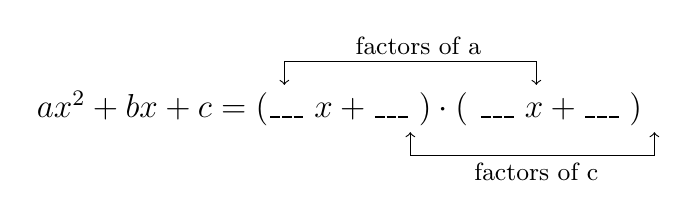
\begin{tikzpicture}
    \node at (0,0) {\large $ax^2 + bx + c = ( \_\_\_ \ x + \_\_\_ \ ) \cdot (\ \_\_\_ \ x + \_\_\_ \ )$};
    % Upper arrow and label
    \draw[<->] (-0.7,0.3) -- (-0.7,0.6) -- (2.5,0.6) -- (2.5,0.3);
    \node at (1,0.8) {\small factors of a};
    % Lower arrow and label
    \draw[<->] (0.9,-0.3) -- (0.9,-0.6) -- (4,-0.6) -- (4,-0.3);
    \node at (2.5,-0.8) {\small factors of c};
\end{tikzpicture}
\end{center}
\textbf{For example,}\ \ $6x^2+5x-4$\\\\
Factors of a (6): (1,6)\tikz[baseline]{\node[draw,circle,inner sep=1pt] {(2,3)};} \ \ Factors of c (-4): (1,-4)(2,-2)\tikz[baseline]{\node[draw,circle,inner sep=1pt] {(-1,4)};}\\
By trying combinations of factors we find: $(2x-1)(3x+4)$

\newpage

\section*{Factoring Examples with Rectangles}
\subsection*{How long is a piece of string?}
Say you have a rectangular yard that you know is 48 square metres in area. You want to measure the lengths of the two sides but all you have is a piece of string of unknown length, which you call $x$. Measuring the yard with your string you find that one side has a length of $x+3$ and the other has a length of $3x-1$. How long is your piece of string?\\

You make a drawing:
\begin{center}
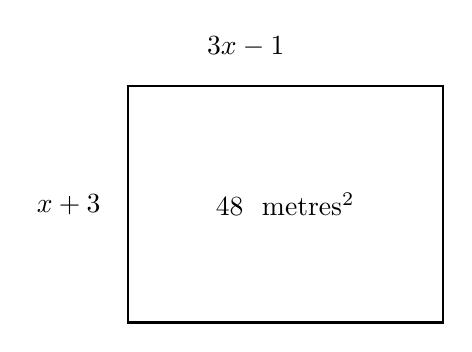
\begin{tikzpicture}[scale=0.5]
\draw[thick] (0,0) -- (0,6) -- (8,6) -- (8,0) -- cycle;
\node at (-1.5,3) {$x+3$};
\node at (3,7) {$3x-1$};
\node at (4,3) {$48$ \ metres$^2$};
\end{tikzpicture}
\end{center}

You write this up as a quadratic equation:
$$(x+3)(3x-1)=48$$
You expand this out into standard form:
$$3x^2-x+9x-3=48 \implies 3x^2+8x-51=0$$
You know that to factorize this you need to find the factors of $ac \ (3\times-51=-153)$ that add to equal $b \ (8)$.\\

You do a prime factor tree to get factors of 153, and you make a table:

\begin{minipage}[t]{0.45\textwidth}
    \centering
    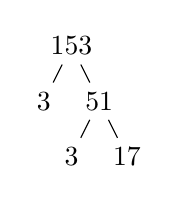
\begin{tikzpicture}
      [level distance=2em,
      level 1/.style={sibling distance=2em},
      level 2/.style={sibling distance=2em}]
      \node {153}
        child {node {3}}
        child {node {51}
          child {node {3}}
          child {node {17}}
        };
    \end{tikzpicture}
\end{minipage}%
\hfill
\begin{minipage}[t]{0.45\textwidth}
    \centering
    \begin{tabular}{rrrrrr}
          factors &  sum &  & factors &  sum & \\
         (-153,1) & -152 &  & (153,1) &  152 & \\
          (-51,3) &  -48 &  & (51,-3) &   48 & \\
          (-17,9) &   -8 &  & (17,-9) &    8 & \\
          (-9,17) &    \textcircled{8} & \leftarrow &
          (9,-17) &   \textcircled{-8} & \leftarrow \\
          (-3,51) &   48 &  & (3,-51) &  -48 & \\
         (-1,153) &  152 &  &(1,-153) & -153 & \\
    \end{tabular}
\end{minipage}

You see there are two ways that you could split $bx$:
$$(3x^2+17x)-(9x-51)=0$$
$$(3x^2-9x)+(17x-51)=0$$

You use the second one because it can be easily factored:
$$3x(x-3)+17(x-3)=0$$

You use the distributive law to get your factors:
$$(3x+17)(x-3)=0$$

You use the null factor law to find the value of $x$:
\begin{table}[h]
    \centering
    \begin{tabular}{rr}
         $3x+17=0$         & $x-3=0$ \\
         $x=\frac{-17}{3}$ & $x=3$
    \end{tabular}
\end{table}

You see that $\frac{-17}{3}$ isn't a valid length, so your string must be 3 metres long.\\

Knowing that, you apply it to the original measurements\\of $(x+3)(3x-1)=48$:

\begin{center}
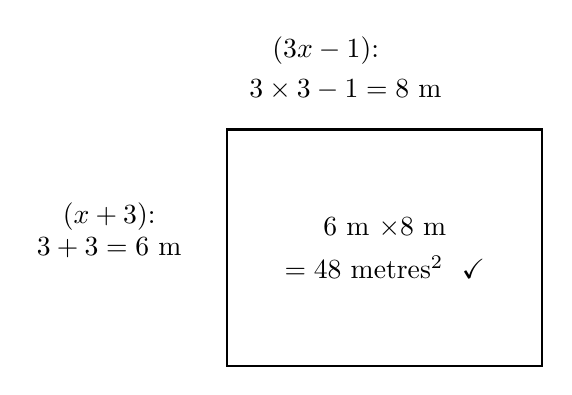
\begin{tikzpicture}[scale=0.5]
\draw[thick] (0,0) -- (0,6) -- (8,6) -- (8,0) -- cycle;
\node at (-3,3.8) {$(x+3)$:};
\node at (-3,3)   {$3+3=6$ m};
\node at (2.5,8) {$(3x-1)$:};
\node at (3,7)   {$3\times3-1=8$ m};
\node at (4,3.5) {$6$ m $\times 8$ m};
\node at (4,2.5) {$=48$ metres$^2$ \ \checkmark};
\end{tikzpicture}
\end{center}

You see that your maths is correct and that the lengths of the sides of your yard are 8 metres by 6 metres.

\subsection*{Another Rectangle:}

A rectangle has an area of 45 square centimetres, and is 4 centimetres longer on one side than the other. What are the lengths of its sides?

As an equation that is: $x(x+4)=45$

Multiplying it out to standard form: $x^2+4x-45=0$

Factor by grouping:\\
\begin{table}[h]
    \centering
    \begin{tabular}{rrrrrr}
          factors & sum &  & factors &  sum & \\
          (-45,1) & -44 &  & (45,-1) &   44 & \\
           (-9,5) &  -4 &  & (15,-3) &   12 & \\
           (-5,9) &  \textcircled{4} & \leftarrow & (9,-5) & \textcircled{4} & \leftarrow \\
          (-15,3) & -12 &  &  (5,-9) &   -4 & \\
          (-3,15) &  12 &  & (3,-15) &  -12 & \\
          (-1,45) &  44 &  & (1,-45) &  -44 & \\
    \end{tabular}
\end{table}
Splitting $bx$ with factors of $ac$ that add to $b$:
$$(x^2-5x)+(9x-45)=0$$
$$(x^2+9x)-(5x-45)=0$$
The first one looks simpler.\\
Factor each binomial: $x(x-5)9(x-5)=0$\\
Distribute: $(x-9)(x-5)=0$\\
\begin{table}[h]
    \centering
    \begin{tabular}{rr}
         $x-5=0$ & $x+9=0$ \\
         $x=5$   & \underbrace{$x=-9$}_{\small{\textrm{not a valid length}}}
    \end{tabular}
\end{table}
The rectangle is $5 \times 9$ cm:
\begin{center}
\begin{tikzpicture}[scale=0.5]
\draw (0,0) -- (9,0) -- (9,5) -- (0,5) -- cycle;
\draw [dashed](5,0) -- (5,5);
\node at (4.5,7){$(x+4)$}
\node at (2.5,6){5 cm}
\node at (7,6){4 cm}
\node at (-1.5,3.5){$(x)$}
\node at (-1.5,2.5){5 cm}
\node at (2.5,2.5){25 cm$^2$}
\node at (7,2.5){20 cm$^2$}
\node at (4.5,-1){25 + 20 = 45 cm$^2$\checkmark}
\end{tikzpicture}
\end{center}

\end{document}